\documentclass[a4paper, 12pt]{beamer} %%%here01

\usetheme{CambridgeUS}
\usecolortheme{beaver}
\usefonttheme{structuresmallcapsserif}


\usepackage[slovene]{babel}
\usepackage[utf8]{inputenc}
\usepackage[T1]{fontenc}
\usepackage{lmodern}
\usepackage{units}
\usepackage{eurosym}
\usepackage{amsmath}
\usepackage{amssymb}
\usepackage{amsthm}
\usepackage{amsfonts}
\usepackage{mathtools}
\usepackage{graphicx}
\usepackage{color}
%\usepackage{url}
\usepackage{enumerate}
\usepackage{enumitem}
\usepackage{pifont}

\definecolor{airforceblue}{rgb}{0.36, 0.54, 0.66}
\definecolor{bostonuniversityred}{rgb}{0.8, 0.0, 0.0}

\newcommand{\Zn}{\mathbb{Z}_n}
\renewcommand{\P}{\mathbb{P}}

\newenvironment{matematika}[1]{
\textcolor{bostonuniversityred}{\underline{\textsc{#1:}}}
}{
}

\title{Algoritem RSA}
\subtitle{Uporaba, prednosti in slabosti}
\author{Benjamin Benčina}
\institute[FMF UL]{Univerza v Ljubljani \\ Fakulteta za matematiko in fiziko \\ Oddelek za matematiko}
\date{\today}

\begin{document}
\titlepage

\begin{frame}{Uvod v kriptografijo}
\begin{itemize}[label=\ding{227}]
\item<1-> Umetnost skrivanja podatkov vsem na očeh.
\item<2-> Tajne združbe, varnostne službe, vojska, dvorci, zločinci, intelektualna elita, znanstveniki, ugankarji, računalniški protokoli...
\item<3-> Kriptanaliza - matematična sestrična tradicionalne kriptografije
\end{itemize}
\end{frame}

\begin{frame}{Kriptografija pred računalniki}
\begin{itemize}[label=\ding{227}]
\item<1-> Tajne pisave, skitala, piktogrami, premetanke...
\item<2-> Cezarjanka ($x \mapsto x + c$)
\item<3-> Vigen\`{e}rov kvadrat (urejena $n$-terica preslikav oblike $x \mapsto x + c_i$; kjer je $n$ dolžina ključa in $i \in [n]$)
\item<4-> Enigma in Alan Turing

\end{itemize}
\end{frame}

\begin{frame}{Kriptografija pred računalniki}
\framesubtitle{Turingove bombe}
\begin{minipage}[b]{0.45\linewidth}
\begin{figure}
\centering
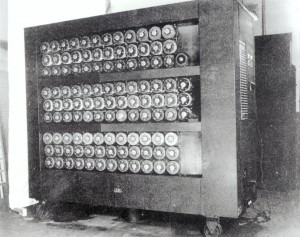
\includegraphics[scale=0.6]{turingbomb}
\caption{Ena od Turingovih bomb}
\label{fig:bomba}
\end{figure}
\end{minipage}
\hfill
\begin{minipage}[b]{0.45\linewidth}
\begin{figure}
\centering
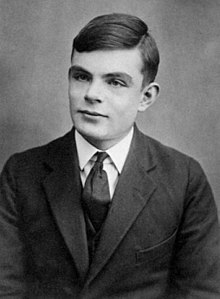
\includegraphics[scale=0.5]{AlanTuring16}
\label{fig:turing}
\caption{Alan Turing, 16 let}
\end{figure}
\end{minipage}
\end{frame}

\begin{frame}{Motivacija}
\begin{itemize}[label=\ding{227}]
\item<1->Ročne šifre so nepraktične, njihova varnost nezanesljiva.
\item<2->Mehanične šifre so drage s preveč dinamičnim algoritmom.
\item<3->Obe vrsti tradicionalnega šifriranja sta proti računalniku skoraj vedno neuporabni.
\end{itemize}
\begin{alertblock}<4->{}
\alert{Potreba po univerzalnem, matematično trdnem in varnem algoritmu.}
\end{alertblock}
\end{frame}

\begin{frame}{1978, ideja je rojena}
\begin{figure}
\centering
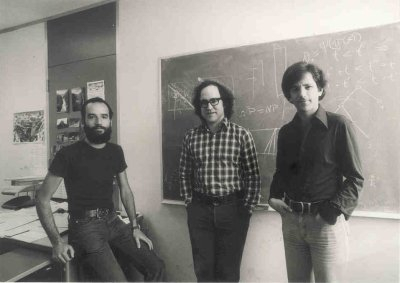
\includegraphics[scale=1.2]{rsa_inventors}
\label{fig:inventors}
\caption{Izumitelji algoritma Ronald \alert{R}ivest (sredina), Adi \alert{S}hamir (levo) in Leonard \alert{A}dleman (desno) po podelitvi patenta, 1983.}
\end{figure}
\end{frame}

\begin{frame}{Matematične osnove}
\framesubtitle{Modularna aritmetika in kolobar $\Zn$}
\begin{block}<1->{}
\begin{matematika}{definicija}
\textbf{Modularna aritmetika} (včasih tudi urna aritmetika) po modulu $n$ je aritmetika omejena s kongruenčno relacijo $a R_n b \iff n | b - a$ .
\newline
\newline
Z drugimi besedami je to aritmetika v kolobarju $\Zn$, tj. je kolobar ostankov pri deljenju celih števil z $n$, kjer je $n$ \textbf{modul}.
\end{matematika}
\end{block}

\begin{block}<2->{}
\begin{matematika}{oznake}
\newline
\begin{itemize}[label=\ding{43}]
\item Operacija $\text{mod: } \mathbb{Z} \times \mathbb{Z} \to \mathbb{Z}$ $(a, b) \mapsto \text{ostanek števila } a \text{ pri deljenju z } b$
\item Relacija $a = b \text{ (mod } n)$ pomeni, da celi števili $a$ in $b$ vrneta isti ostanek pri deljenju z $n$, oziroma mod($a$,$n$) = mod($b$,$n$).
\end{itemize}
\end{matematika}
\end{block}
\end{frame}


\begin{frame}{Matematične osnove}
\framesubtitle{Funkcija $\varphi$ in Eulerjev izrek}
\begin{block}<1->{}
\begin{matematika}{definicija}
Eulerjeva funkcija $\varphi$($n$) vrne število vseh pozitivnih celih števil manjših od $n$, ki so $n$ tuja.
\newline
\newline
$\varphi$($n$) $=$ \#\{ $a \in \mathbb{N}$; $a \leq n$, gcd($a$, $n$)$=1$\}
\end{matematika}
\end{block}

\begin{block}<2->{}
\begin{matematika}{eulerjev izrek}
Če sta si števili $x$ in $n$ tuji, velja:
\[
x^{\varphi(n)} = 1 \text{ (mod }n)
\]
\end{matematika}
\end{block}

\begin{block}<3->{}
\begin{matematika}{opomba}
$\varphi(p) = p-1$, če je $p$ praštevilo.
\end{matematika}
\end{block}
\end{frame}

\begin{frame}{Matematične osnove}
\framesubtitle{Polinomi in številski sistemi}
\begin{block}<1->{}
\begin{matematika}{definicija}
Polinom $f$ je formalna vsota $f(X) = a_0 + a_1X + \cdots + a_nX^n.$ $X$ imenujemo \emph{spremenljivka}, številom $a_i$ pravimo \emph{koeficienti}, $n$ pa je \emph{stopnja} polinoma. Vsak polinom porodi \textbf{polinomsko funkcijo}.
\end{matematika}
\end{block}

\begin{block}<2->{}
\begin{matematika}{definicija}
Število je zapisano v $n$-iškem \textbf{številskem sistemu}, $n \geq 2$, če je enako vrednosti neke polinomske funkcije iz $\Zn$ izračunane za $X = n$ in je $a_i$ števka tega števila na $i$-tem mestu, šteto od desne proti levi od $0$ naprej.
\end{matematika}
\end{block}
\end{frame}

\begin{frame}{Kako deluje?}
\begin{itemize}[label=\ding{227}]
\item<1-> Izberemo si dve različni praštevili $p$ in $q$.
\item<2-> Izračunamo $n = p \cdot q$ in $\phi(n) = \phi(p) \cdot \phi(q) = (p-1) \cdot (q-1).$
\item<3-> Izberemo naključen $e$, za katerega velja gcd($e, \phi(n)) = 1$.
\item<4-> Z razširjenim Evklidovim algoritmom poiščemo $d$, ki je multiplikativen inverz za $e$ v kolobarju $\mathbb{Z}_{\phi(n)}$. Drugače: $e \cdot d = 1 \text{ (mod } \phi(n))$.
\item<5-> Sporočilo $m$ šifriramo tako: $c = m^e \text{ mod } n$.
\item<6-> Skrito sporočilo dešifriramo tako: $m = c^d \text{ mod } n$.
\end{itemize}
\end{frame}

\begin{frame}{Zakaj deluje?}
\begin{block}<1->{}
\begin{matematika}{izrek}
Naj bo $n \in \mathbb{Z}$ produkt samih različnih praštevil in naj bosta $d, e\in \mathbb{N}$ taki, da za $\forall p \in \mathbb{P}$ velja $(p-1) | (d \cdot e - 1)$. Tedaj:
\newline
\[
\forall a \in \mathbb{Z}: \text{ } a^{d \cdot e} = a \text{ (mod }n)
\]
\end{matematika}
\end{block}
\end{frame}

\begin{frame}{Kodiranje zaporedja znakov v števila}
\begin{itemize}[label=\ding{227}]
\item<1-> Izračunamo moč množice znakov, ki bi jih radi kodirali. Naj bo to število $m$.
\item<2-> Vsakemu znaku iz te množice priredimo vrednost iz množice $\mathbb{Z}_m$.
\item<3-> Preštejemo število znakov, ki bi jih radi kodirali. Naj bo to število $j$.
\item<4-> Zaporedje znakov razbijemo v take kose, da je $j$ vsakega kosa strogo manj od $\log_{m}(n)$.
\item<4-> Nato sestavimo polinom $f(X) = a_0 + a_1 \cdot X + \cdots + a_j \cdot X^j$. 
\item<5-> Naše iskano število je vrednost polinomske funkcije tega polinoma izračunane za $x = m$.
\end{itemize}
\end{frame}

\begin{frame}{Načrt napada}
Iz matematičnega vidika se da algoritem napasti na treh točkah:
\begin{itemize}[label=\ding{227}]
\item<1-> določimo praštevili $p$ in $q$ modula $n$, nato izračunamo $\phi(n)$ in posledično $d$;
\item<2-> določimo $\phi(n)$ direktno iz javnega ključa $\{ e, n \}$ in posledično $d$;
\item<3-> določimo $d$ direktno iz javnega ključa $\{ e, n \}$.
\end{itemize}
\begin{block}<4->{}
Pokazati se da, da je zahtevnost drugega in tretjega pristopa enaka zahtevnosti faktorizacije števila $n$. Torej je varnost algoritma proti matematičnim napadom določena s časom potrebnim za faktorizacijo števila $n$ na $p$ in $q$.
\end{block}
\end{frame}

\begin{frame}{Napad 1:}
\framesubtitle{Faktorizacija $n$, če poznamo $\phi(n)$}
\begin{itemize}[label=\ding{227}]
\item<1-> Naj bo $n = p \cdot q$ in $\phi(n)$ znano število.
\item<2-> Velja $\phi(n) = (p-1) \cdot (q-1) = p \cdot q - (p + q) + 1$, torej poznamo tako $p \cdot q = n$ kot $p + q = n + 1 - \phi(n)$.
\item<3-> Torej po Vietovih formulah vemo, da velja $x^2 - (p-q) \cdot x + p \cdot q = (x-p) \cdot (x-q).$
\item<4-> $p$ in $q$ sta očitno ničli te kvadratne funkcije in zato lahko izračunljivi po splošni formuli.
\end{itemize}
\end{frame}

\begin{frame}{Napad 2:}
\framesubtitle{Kaj če sta $p$ in $q$ blizu skupaj?}
\begin{itemize}[label=\ding{227}]
\item<1-> Denimo, da vemo, da je razlika števil $p$ in $q$ majhna. Potem je $n$ lahko faktorizirati s \emph{Fermatovo faktorizacijsko metodo}.
\item<2-> Brez izgube splošnosti lahko rečemo, da $p > q$. Potem $n = (\frac{p+q}{2})^2 - (\frac{p-q}{2})^2$.
\item<3-> Ker sta $p$ in $q$ "blizu", je $s=\frac{p-q}{2}$ majhno število, $t = \frac{p+q}{2}$ pa je le malce večje od $\sqrt{n}$, $t^2 - n = s^2$ pa je popoln kvadrat.
\item<4-> Za $t$ jemljemo $\lceil \sqrt{n} \rceil + k$, kjer $k \in \{ 0, 1, \dots \}$, dokler $t^2 - n$ ni popoln kvadrat.
\item<5-> Potem velja: $p = t + s$ in $q = t - s$.
\end{itemize}
\end{frame}

\begin{frame}{Napad 3:}
\framesubtitle{Faktorizacija $n$, če poznamo $d$, oz. napad na skupen modul}
Pokažimo, da je iskanje $d$ vsaj tako težko kot faktorizacija $n$. Recimo, da $d$ imamo. Naj bo $m = d \cdot e - 1$. Torej velja $a^m = 1 \text{ (mod }n)$.
\begin{block}<2->{}
\begin{matematika}{algoritem}
\begin{itemize}[label=\ding{227}]
\item<2->  Če je $m$ sod in $a^{m/2} = 1 \text{ (mod }n)$ za več naključnih $a$-jev, nastavimo $m = \frac{m}{2}$. Ponavljamo dokler so pogoji na $m$ zadoščeni.
\item<3-> Izberemo naključen $a$ in izračunamo $g = \text{gcd}(a^{m/2} -1, n)$.
\item<4-> Če je $g$ pravi delitelj $n$, smo našli vrednost in zaključimo. Drugače nazaj na drugi korak.
\end{itemize}
\end{matematika}
\end{block}
\begin{block}<5->{}
\alert{Dve osebi naj zato nikoli ne uporabljata istega $n$.}
\end{block}
\end{frame}

\begin{frame}{Napad 4:}
\framesubtitle{Chosen-Ciphertext Attack}
\begin{itemize}[label=\ding{227}]
\item<1-> Preprost napad, ki temelji na standardni velikosti blokov sporočila.
\item<2-> Napadalec določi množico možnih sporočil, izbere najbolj verjetne, jih zakodira z javnim ključem in nato primerja šifro (oz. po ang. Ciphertext).
\item <3->
Rešitve:
\begin{itemize}[label=\ding{226}]
\item<4-> Sporočilo \emph{posolimo}, tj. mu na začetek vsakega bloka dodamo dogovorjeno število naključnih znakov.
\item<5-> Poskrbimo, da je naša izbira javnega ključa takšna, da je množica možnih sporočil kar se da velika.
\end{itemize}
\end{itemize}
\end{frame}

\begin{frame}{Napad 5:}
 \framesubtitle{Napad na majhen šifrirni eksponent $e$}
Mogoče se zdi, da je zaradi računske učinkovitosti pametno izbrati čim manjši $e$.
\newline
\begin{block}<2->{}
\alert{NAPAKA!}
\end{block}
\begin{itemize}[label=\ding{227}]
\item<3-> Če ima tudi sporočilo $m$ majhno vrednost, torej da $m^e < n$, potem tudi $c = m^e$. Torej lahko iz šifre $c$ dobimo izvorno sporočilo zlahka tako: $m = c^{1/e}$.
\end{itemize}
\begin{block}<4->{}
Rešitev: premajhno sporočilo spet lahko \emph{posolimo}, da povečamo $m^e > n$, poleg tega pa je vedno pametno izbrati večji $e$.
\end{block}
\end{frame}

\begin{frame}{Napad 6:}
\framesubtitle{Napad na majhen prostor sporočil}
\begin{itemize}[label=\ding{227}]
\item<1-> Če je slika preslikave šifriranja pri izbranem javnem ključu premajhna, lahko napadalec sistem očitno učinkovito napade že s surovo silo (\emph{brute force}), saj lahko preprosto izračuna vse šifrirane nize in jih primerja s prestreženim.   
\item<2-> Na velikost prostora sporočil lahko vpliva veliko parametrov, predvsem izbira praštevil $p$ in $q$, izbira $e$ ter posledično "izbira" $d$.
\item<3-> Ta napad je zato kombinacija tehnik Chosen-Ciphertext napada, napada na majhen šifrirni eksponent in naslednjega napada.
\end{itemize}
\begin{block}<4->{}
Splošna rešitev je spet naključno \emph{soljenje} sporočila in predvsem pametna izbira ključev.
\end{block}
\end{frame}

\begin{frame}{Napad 7:}
\framesubtitle{Napad na majhen dešifrirni eksponent $d$}
Zopet bi se mogoče zdelo smiselno izbrati čim manjši $d$ v imenu računske učinkovitosti.
\newline
\begin{block}<2->{}
\alert{NAPAKA!}
\end{block}
\begin{block}<3->{}
Kriptograf Michael J. Wiener je pokazal, da se da $d$ da učinkovito določiti, če $d < \frac{1}{3} \cdot n^{1/4}$ in če za praštevili $p$ in $q$ velja $q < p < 2 \cdot q$.
\end{block}
\begin{block}<4->{}
Rešitev je očitna: eksponent $e$ moramo pazljivo izbrati tako, da $d > \frac{1}{3} \cdot n^{1/4}$
\end{block}
\end{frame}

\begin{frame}{Napad 8:}
\framesubtitle{Cikličen napad}
CIkličen napad je idejno najpreprostejši napad na algoritem RSA poleg seveda \emph{brute force} napada:
\begin{itemize}[label=\ding{227}]
\item<1-> Šifro z javnim ključem še enkrat šifriramo. Ta korak ponavljamo, dokler ne šifriramo dobljenega števila nazaj v izvorno šifro.
\item<2-> Ko se to zgodi, pogledamo eno šifriranje nazaj, to število mora biti izvirno sporočilo.
\end{itemize}
\begin{block}<3->{}
Ta napad je ob pravilni izbiri javnega ključa časovno ekvivalenten \emph{brute force} napadu.
\newline
Njegova edina dobra lastnost je, da je odporen na \emph{soljenje} sporočila, 
\end{block}
\end{frame}

\begin{frame}{Uporaba}
\begin{itemize}[label=\ding{227}]
\item<1-> OpenSSH protokol.
\item<2-> Če obrnemo vlogo prejemnika in pošiljatelja, lahko algoritem RSA nadomešča t.i. kriptografsko \emph{hash funkcijo} pri preverjanju istovetnosti.
\item<3-> Zaradi visoke računske zahtevnosti je algoritem pogosto prepočasen za pošiljanje podatkov v realnem času, zato pa pogosto igra vlogo anonimizatorja predaje ključa za hitrejše simetrične šifre, namesto recimo \emph{Diffie-Hellmanove izmenjave ključa}.
\end{itemize}
\end{frame}

\begin{frame}
\begin{block}{}
\LARGE
\centering
HVALA ZA POZORNOST!
\end{block}
\end{frame}

\end{document}